\documentclass[border={0pt 0pt 0pt 0pt},convert={density=300,outext=.png}]{standalone}

\usepackage{tikz}
\usepackage{pgf}
\usepackage{subcaption}
% \usepackage[margin=0.5pt]{geometry}
\usetikzlibrary{calc}   % coordinate calculation

\newcommand{\defstuff} {
  \def \step {1}
  \def \cc {\step/2}  % center of cell
  \coordinate (offset) at ($(\cc,\cc)$);
}

\newcommand{\drawgrid}[1] {
  \draw[step=\step, color=gray] (0,0) grid ($#1$); % draw the grid, base at #1
}

\newcommand{\drawrobots}[1] {
    \foreach \coord in #1 {
      \coordinate[at=\coord, name=A];
      \draw ($(A) + (offset)$) circle ({\cc*0.8});
    }
}

\newcommand{\drawarrows}[1] {
    \foreach \a/\b in #1 {
      \coordinate[at=\a, name=A];
      \coordinate[at=\b, name=B];
      \draw[->, color=darkgray] ($(A) + (offset)$) -- ($(B) + (offset)$);
    }
}

\newcommand{\spacee}[3] {
  \begin{tikzpicture}[thick, scale=0.6]
    \defstuff
    \drawgrid{#1}
    \drawrobots{#2}
    \drawarrows{#3}
  \end{tikzpicture}
}


\begin{document}

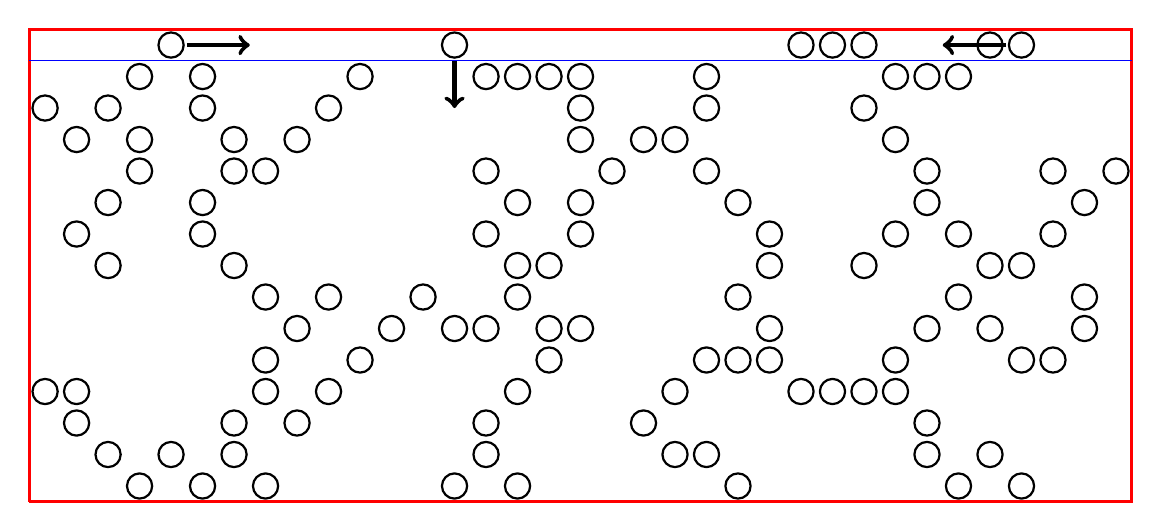
\begin{tikzpicture}[thick, scale=0.4]
\defstuff
\drawrobots{{(22, 19),(2, 22),(14, 18),(5, 18),(26, 17),(17, 23),(15, 19),(18,
20),(8, 15),(7, 10),(3, 23),(8, 21),(9, 16),(24, 24),(31, 24),(10, 23),(13,
10),(2, 17),(17, 18),(1, 12),(8, 12),(2, 11),(34, 20),(30, 11),(28, 15),(10,
14),(11, 15),(15, 16),(26, 24),(15, 13),(27, 21),(13, 15),(29, 23),(28,
12),(15, 23),(17, 21),(20, 21),(22, 16),(22, 10),(7, 20),(6, 11),(15, 10),(31,
17),(17, 22),(16, 23),(21, 11),(26, 13),(29, 16),(9, 13),(30, 15),(28, 11),(31,
14),(23, 17),(29, 10),(7, 13),(14, 12),(30, 17),(19, 12),(3, 10),(23, 18),(21,
14),(1, 21),(3, 21),(6, 12),(16, 14),(6, 17),(5, 23),(17, 15),(16, 17),(21,
20),(2, 19),(32, 20),(28, 23),(3, 20),(22, 14),(23, 15),(14, 23),(30, 24),(19,
21),(7, 14),(21, 23),(28, 20),(5, 10),(31, 10),(25, 24),(20, 11),(1, 18),(25,
13),(7, 16),(4, 24),(0, 22),(12, 16),(9, 22),(6, 21),(5, 19),(24, 13),(28,
19),(29, 18),(27, 14),(6, 20),(32, 14),(33, 15),(16, 15),(5, 22),(20, 13),(27,
23),(17, 19),(13, 24),(1, 13),(33, 16),(27, 13),(4, 11),(23, 14),(14, 20),(15,
17),(14, 11),(21, 22),(27, 18),(26, 22),(0, 13),(32, 18),(33, 19),(14, 15)}}
\draw[very thick,red] (0,10) -- (35,10) -- (35,25) -- (0,25) -- (0,10);
\draw[ultra thick,->] (5,24.5) -- (7,24.5);
\draw[ultra thick,->] (31,24.5) -- (29,24.5);
\draw[ultra thick,->] (13.5,24) -- (13.5,22.5);
\draw[thin,blue] (0,24) -- (35,24);
\end{tikzpicture}
$BB(t)$

\end{document}
